\section{Distributed constructions and the three moves}\label{sec:moves}

\begin{inwords}
To convert logarithmic decoupling into a tensor network, we track how
ownership of the chain's site registers is transferred among a finite set of
\emph{parties}. Each party holds a collection of registers (tensor factors),
which may include complete copies of the ground vector prepared privately. A
\emph{gate} is a linear contraction applied to the registers of a small
number of parties. A gate is \emph{private} if it acts on a single party's
registers; private gates are free. A non-private gate is charged through
only two combinatorial quantities: how many parties it involves, and how
many non-private gates each party participates in over the entire protocol.
In addition, every non-private gate must admit a \emph{polynomial
expansion}: it must be a sum of polynomially many terms, each a composition
of private contractions, preparations of normalised bipartite vectors shared
by two parties, contractions against normalised bipartite covectors shared by
two parties, and transfers of polynomial-dimensional registers. Crucially,
the Hilbert-space dimensions of the private registers and of the shared
bipartite vectors are unrestricted.

Separating private Hilbert-space dimension from gate participation count is
the key mechanism of the protocol: as shown in Section~\ref{sec:compression},
the final physical density matrix of any such distributed construction can be
compressed into a tensor network on the party graph with polynomial bond
dimension, regardless of the dimensions of the private registers or shared
resources. One party may therefore prepare the exact ground vector $\Om$
privately, and pairs of parties may share arbitrarily entangled bipartite
states, provided each party takes part in only a bounded number of
non-private gates.

A \emph{sheet} is a complete set of chain registers
$\cH_\Lam=\bigotimes_{x\in\Lam}\C^q$ equipped with an assignment of a party
(its owner) to each site; its reference vector is a copy of $\Om$ placed on
those registers in canonical site coordinates (changing ownership relabels
which party holds a site register without permuting sites). Three elementary
moves modify the ownership assignment of one or two sheets while keeping the
actual state vector within $O(L^{-p/2})$ of the tensor product of the
reference vectors. A \emph{birth} hands a set $T$ of sites from a party
$P_\circ$ to another party $Q_\circ$ when $T$ carries little mutual
information with the sites $P_\circ$ does not own; a \emph{death} hands $T$
back when the same condition holds after the move; and a \emph{two-sheet
exchange} swaps the two ownership assignments inside an interval $Y$ under
the analogous information condition, without moving any register between
parties.
\end{inwords}

\precisely
A \emph{distributed construction} of size parameter $L$ consists of a
finite set of parties, each initialised with a finite-dimensional register
space in a normalised product state, together with a sequence of gates,
each a linear contraction between specified input and output register
spaces of the participating parties while all other registers act as
spectators. Registers to be discarded are retained until a final partial
trace. An \emph{allowed monomial} is a composition of private
contractions, preparations of normalised vectors shared between two
participating parties, contractions against normalised covectors shared
between two participating parties, and identity transfers of registers of
uniformly polynomial dimension. A non-private gate is \emph{admissible} if
it is a sum of uniformly polynomially many allowed monomials with
uniformly polynomially bounded scalar coefficients, each monomial
containing a bounded number of shared vectors, shared covectors, and
transfers; a contraction within $L^{-a}$ of such a sum, for a fixed $a>0$,
is also admissible after rescaling by $1+L^{-a}$. A \emph{bounded change}
is a sequence of a bounded number of admissible gates on a bounded number
of parties.

A sheet is $\cH_\Lam=\bigotimes_{x\in\Lam}\C^q$ with an owner assigned to
each site; its reference vector is $\Om$ placed in these registers.

\begin{lemma}[Birth and death]\label{lem:birth}
In a sheet, let $T$ be a set of sites owned by $P_\circ$, and let
$E=\{x:\text{the owner of }x\text{ is not }P_\circ\}$ and
$U=\Lam\setminus(T\cup E)$. If $I_\Om(T:E)\le L^{-2p}$, then changing the
owner of $T$ from $P_\circ$ to any party $Q_\circ$ (a \emph{birth}) is a bounded
change involving $P_\circ$ and $Q_\circ$ only, consisting of private maps and one
shared normalised vector, with reference-vector error at most $L^{-p}$.
The reverse change (a \emph{death}, returning $T$ from $Q_\circ$ to
$P_\circ$) is a bounded change with the same error whenever the
ownership and information conditions hold in the sheet \emph{after} the
death; it uses one shared normalised covector instead.
\end{lemma}
\begin{proof}
Let $V,s,s'$ be given by Lemma~\ref{lem:splitting} for $(T,U,E)$, and put
$\mathcal V=\id_{TE}\otimes V$ and $\Pi=\ket s\bra s_{T\cB_T}\otimes\id_{E\cB_E}$.
Before the birth, all of $T\cup U$ is owned by $P_\circ$. At $P_\circ$, apply $V$ on $U$; contract
$T\cB_T$ privately against $\bra s$ (both registers are held by $P_\circ$); supply the shared
vector $s$ on $T\cB_T$ with $T$ now owned by $Q_\circ$ and $\cB_T$ retained by
$P_\circ$; and apply $V^\dagger$ at $P_\circ$. The composite map is the Hermitian
contraction $B=\mathcal V^\dagger\Pi\mathcal V$, which satisfies
$\norm{(B-\id)\Om}\le\norm{(\Pi-\id)\mathcal V\Om}=\norm{(\Pi-\id)(\mathcal V\Om-s\otimes s')}\le L^{-p}$.
For a death, apply $V$ at $P_\circ$, contract $T\cB_T$ using the shared covector $\bra s$
held across $Q_\circ$ and $P_\circ$, re-insert $s$ privately at $P_\circ$, and
apply $V^\dagger$: this implements the same operator $B$ with reversed ownership.
\end{proof}

\begin{figure*}[t]
\centering
\begin{adjustbox}{max width=\linewidth}
\(\displaystyle \begin{quantikz}
    \lstick{$T$ at $P_\circ$} & & & \gate[2]{\langle s|} & \gate[2]{|s\rangle}\setwiretype{n} & \setwiretype{q} & & & \rstick{$T$ at $Q_\circ$} \\
    \setwiretype{n} & & \gate[2][1.5cm]{V}\gateoutput{$\mathcal B_T$} & \setwiretype{q} & \setwiretype{n} & \setwiretype{q} & \gate[2][1.5cm]{V^{\dagger}}\gateinput{$\mathcal B_T$} & \setwiretype{n} & \\
    \lstick{$U$ at $P_\circ$} & & \gateoutput{$\mathcal B_E$} & & & & \gateinput{$\mathcal B_E$} & & \rstick{$U$ at $P_\circ$} \\
    \lstick{$E$} & & & & & & & & \rstick{$E$}
  \end{quantikz}\)

\end{adjustbox}
\caption{The birth circuit, read left to right: $V$ splits the buffer, $\langle s|$ closes $T$ and its purifier, a fresh pair $s$ re-emits them with $T$ held by the new owner, and $V^\dagger$ recombines.}\label{fig:qc-birth}
\end{figure*}

\begin{figure*}[t]
\centering
\begin{adjustbox}{max width=\linewidth}
\(\displaystyle \begin{quantikz}
    \lstick{$T\ (Q_\circ)$} & & & \gate[2]{\langle s|}\gategroup[2,steps=1,style={draw=none,inner sep=0pt},label style={label position=below,anchor=north,yshift=-0.15cm}]{\scriptsize shared $Q_\circ,P_\circ$} & \gate[2]{|s\rangle}\gategroup[2,steps=1,style={draw=none,inner sep=0pt},label style={label position=below,anchor=north,yshift=-0.15cm}]{\scriptsize private at $P_\circ$}\setwiretype{n} & \setwiretype{q} & & & \rstick{$T\ (P_\circ)$} \\
    \setwiretype{n} & & \gate[2]{V} & \setwiretype{q} & \setwiretype{n} & \gate[style={draw=none,inner xsep=1pt}]{\mathcal B_T} & \gate[2]{V^{\dagger}} & \setwiretype{n} & \\
    \lstick{$U\ (P_\circ)$} & & & & & & & & \rstick{$U\ (P_\circ)$} \\
    \lstick{$E$} & & & & & & & & \rstick{$E$}
  \end{quantikz}\)

\end{adjustbox}
\caption{The death circuit: the same operator with the ownership reversed, using the shared covector $\langle s|$ across the two owners and a private re-insertion of $s$.}\label{fig:qc-death}
\end{figure*}

\begin{lemma}[Two-sheet exchange]\label{lem:exchange}
Consider two sheets and an interval $Y\subseteq\Lam$. Inside $Y$, exchange
the two ownership assignments (sheet 1 at $x\in Y$ receives the owner sheet 2
had, and conversely); outside $Y$, keep both assignments unchanged. Let $P_\circ$ be a party, and set
\[
\begin{split}
 &Z=\{x:\text{the two owners of }x\text{ are not both }P_\circ\},\\
 &T=Z\cap Y,\quad E=Z\setminus Y,\quad U=\Lam\setminus Z .
\end{split}
\]
If $I_\Om(T:E)\le L^{-2p}$, the exchange is implemented by relabelling
registers (no register changes party) together with private contractions at
$P_\circ$, with error at most $4L^{-p}$ between the tensor products of the old and
new reference vectors.
\end{lemma}
\begin{proof}
Let $\mathcal R$ relabel the two sheets inside $Y$: this is a private identification
of tensor factors because the new owner of sheet 1 at $x\in Y$ coincides with the old
owner of sheet 2 at $x$. In canonical site coordinates, $\mathcal R$ acts as the
swap $F_{Y}$ exchanging the two sheets on $Y$. All registers of $U$ on both sheets
are held by $P_\circ$ both before and after $\mathcal R$. Let $V,s,s'$ be given by
Lemma~\ref{lem:splitting} for $(T,U,E)$, put $\mathcal V=\id_{TE}\otimes V$, and
define $D_U=(V^{\otimes2})^\dagger F_{\cB_T}V^{\otimes2}$ on the two copies of
$U$; this is a private contraction at $P_\circ$ obtained by applying $V$ to both copies, swapping the
two $\cB_T$ factors, and applying $V^\dagger\otimes V^\dagger$. Writing $A=Y\cap U$, apply the private swap $F_A$ after
$\mathcal R$ and then apply $D_U$. Since
$Y=T\sqcup A$, the net action on the two copies in canonical coordinates is
\[
 D_UF_AF_Y=D_UF_T=(\mathcal V^{\otimes2})^\dagger F_{T\cB_T}\mathcal V^{\otimes2},
\]
because $F_T$ acts outside $U$ and commutes with $V^{\otimes2}$. Put
$\zeta=s\otimes s'$ and $\delta=\norm{\mathcal V\Om-\zeta}\le L^{-p}$. Then
$\norm{(\mathcal V\Om)^{\otimes2}-\zeta^{\otimes2}}\le2\delta$, $\zeta^{\otimes2}$
is invariant under $F_{T\cB_T}$ (which swaps two identical factors $s$), and
$(\mathcal V^{\otimes2})^\dagger\mathcal V^{\otimes2}=\id$, so
\[
\begin{split}
 &\bigl\|(\mathcal V^{\otimes2})^\dagger F_{T\cB_T}\mathcal V^{\otimes2}\Om^{\otimes2}-\Om^{\otimes2}\bigr\|\\
 &\qquad\le\norm{(F_{T\cB_T}-\id)\bigl((\mathcal V\Om)^{\otimes2}-\zeta^{\otimes2}\bigr)}\le4\delta .
\end{split}
\]
In canonical coordinates both the old and new two-sheet reference vectors equal
$\Om\otimes\Om$ (since sheet registers are relabelled rather than moved), completing the proof.
\end{proof}

\begin{figure*}[t]
\centering
\begin{adjustbox}{max width=\linewidth}
\(\displaystyle \begin{quantikz}
    \lstick{$T^{(1)}$} & & \swap{3} & & & \rstick{$T^{(1)}$} \\
    \setwiretype{n} & \gate[2][1.5cm]{V}\gateoutput{$\mathcal B_T$} & \setwiretype{q} & \swap{3} & \gate[2][1.5cm]{V^{\dagger}}\gateinput{$\mathcal B_T$} & \setwiretype{n} \\
    \lstick{$U^{(1)}$} & & & & & \rstick{$U^{(1)}$} \\
    \lstick{$T^{(2)}$} & & \targX{} & & & \rstick{$T^{(2)}$} \\
    \setwiretype{n} & \gate[2][1.5cm]{V}\gateoutput{$\mathcal B_T$} & \setwiretype{q} & \targX{} & \gate[2][1.5cm]{V^{\dagger}}\gateinput{$\mathcal B_T$} & \setwiretype{n} \\
    \lstick{$U^{(2)}$} & & & & & \rstick{$U^{(2)}$}
  \end{quantikz}\)

\end{adjustbox}
\caption{The exchange correction on the two sheets: after renaming the registers inside $Y$, the common owner applies $V$ to both buffers, swaps the two purifying factors, and applies the adjoints, which realizes the partial swap on $T$ up to $4L^{-p}$.}\label{fig:qc-exchange}
\end{figure*}

\begin{remark}
In the two-dimensional source \cite{PP}, the analogous ownership moves carry
encoded holes and tags at trijunctions where three owners meet. On a line, the
closures of intervals with distinct owners meet only at two-party interfaces, so
no trijunctions occur and no boundary encodings are required. This is the first of
two reasons why the adaptive patch constraints of \cite[Section~4]{PP} are
unnecessary in one dimension.
\end{remark}

\section{The sweep protocol}\label{sec:sweep}

\begin{inwords}
We now schedule the ownership moves across the chain. Divide $\Lam$ into
consecutive blocks of $t=20w$ sites, where $w=\lceil D_{24}\log L\rceil$ is
the logarithmic decoupling distance of Lemma~\ref{lem:logsep}; the final
block absorbs the remainder and has length between $3t$ and $4t$. Initially,
a single remainder party $R_0$ owns the entire chain. At the start of step $k$,
the ownership word reads
\[
 P_1\,|\,P_2\,|\cdots|\,P_k\,|\,R_k ,
\]
where each party $P_i$ owns block $B_i$ and the remainder party $R_k$ owns
the rest of the chain. Two births inside $R_k$, both permitted because they
leave a buffer of width $w$ separating them from all other owners, create
the next remainder party $R_{k+1}$ on everything beyond block $B_{k+1}$
(plus a $w$-buffer) and the next block owner $P_{k+1}$ on the interior of
block $B_{k+1}$. What remains under $R_k$'s ownership are two buffer bands of
width $w$: one wedged between $P_k$ and $P_{k+1}$, and the other wedged
between $P_{k+1}$ and $R_{k+1}$. Handing these two buffer bands over to
their neighbouring owners is the only nontrivial step of the sweep.

Why can a buffer band $A$ wedged between two distinct owners $C$ (on the
left) and $B$ (on the right) not simply die into $B$? Because $A$ touches
$C$ directly, it has zero separation from a non-$B$ owner, so the
decoupling hypothesis of Lemma~\ref{lem:birth} is not available. To dissolve the band without
ever moving a region near a third party, we use an auxiliary sheet \cite{PP}
in which the interface is pre-wrapped inside nested buffers of $A$, $B$, and
$C$; the sequence transplants verbatim from the edge construction of
\cite{PP}. In units of the band width $w$, with the band $A$ occupying $0<x<1$,
$C$ to its left, and $B$ to its right:
\begin{enumerate}[leftmargin=2em,itemsep=0pt]
\item Prepare a fresh auxiliary copy of the ground vector held entirely by
$C$. On this auxiliary sheet, birth $B$ on $(-6,-1)$, then birth $A$ on
$(-5,-2)$, and then birth $C$ on $(-4,-3)$. The auxiliary ownership word is
now $C\,|\,B\,|\,A\,|\,C\,|\,A\,|\,B\,|\,C$.
\item Exchange the main and auxiliary sheets inside the window
$Y=(-7,-\tfrac72)$. Both endpoints of $Y$ lie inside regions owned by $C$ on
both sheets, and all non-$C$ intervals inside $Y$ are separated from all
non-$C$ intervals outside $Y$ by a margin of width at least $w$. After the
exchange, the main sheet reads $C\,|\,B\,|\,A\,|\,C\,|\,A\,|\,B$ with
interfaces at $-6,-5,-4,0,1$, and the auxiliary sheet is retired.
\item On the main sheet, every subsequent move is flanked by a single owner
on both sides: the $C$ band $(-4,0)$ is flanked by $A$ on $(-5,-4)$ and
$(0,1)$, so it dies into $A$; the merged $A$ band $(-5,1)$ is flanked by $B$
on $(-6,-5)$ and $(1,2)$, so it dies into $B$, reducing the word to $C\,|\,B$
with interface at $-6$. Finally, birth $C$ on $(-3,0)$ inside $B$ and let
the $B$ band $(-6,-3)$ die into $C$: the interface returns to $x=0$ with the
original band $(0,1)$ absorbed into $B$.
\end{enumerate}
Every move in this sequence modifies an interval separated by distance at
least $w$ from all third-party owners, so Lemma~\ref{lem:logsep} supplies
the decoupling bound required by Lemma~\ref{lem:birth} or
Lemma~\ref{lem:exchange}. Only the three parties $A,B,C$ participate. Because
each party is born once, dissolves the buffer bands on its two sides once,
and is otherwise a spectator, every party participates in a uniformly bounded
number of gates.

Why use a linear sweep rather than a multiscale dyadic hierarchy? Because
the compressed party network must ultimately be routed onto the
one-dimensional chain. Each link of the party network connects two parties,
and every link crossing a given cut of the chain multiplies the bond
dimension across that cut. In a dyadic hierarchy of intervals, every scale
contributes a link across the midpoint of the chain (the interval tree has
cutwidth $\log L$), which would inflate the bond dimension to
$L^{O(\log L)}$. In the linear sweep, every non-private gate links parties
associated with blocks at most two apart, so only $O(1)$ links cross any cut
of the chain.
\end{inwords}

\precisely
Fix $p=12$. Let $D_{24}$ be the constant of Lemma~\ref{lem:logsep} with
exponent $2p=24$ and $k_0=1$, and put
\begin{equation}\label{eq:blocks}
\begin{split}
 &w=\lceil D_{24}\log L\rceil,\qquad t=20w,\\
 &k_*=\max\{k\ge0:\ L-kt\ge 3t\},
\end{split}
\end{equation}
with blocks $B_i=[(i-1)t+1,\,it]$ for $1\le i\le k_*$ and final block
$B_{k_*+1}=[k_*t+1,L]$ of length in $[3t,4t)$. We assume $L$ is large enough
that $t\ge 20$ and $k_*\ge0$ (smaller $L$ are treated directly in Section~\ref{sec:routing}).
For a band $[a,a+w)$ with $C$ owning $[a-8w,a)$ and $B$ owning
$[a+w,a+2w)$ (and possibly further sites), write $x=(\cdot-a)/w$ for the scaled
coordinate.

\begin{construction}[Band dissolution]\label{con:band}
Suppose the main sheet reads $C\,|\,A\,|\,B$ near $a$: $C$ owns $x<0$ down to at
least $x=-8$, $A$ owns $0<x<1$, and $B$ owns $x>1$ up to at least $x=2$, where
$A,B,C$ are three distinct parties. Perform the following sequence of moves:
\begin{enumerate}[leftmargin=2em]
\item[(i)] Prepare an auxiliary sheet as a fresh copy of $\Om$ held entirely
by $C$ (a private initialisation). On this auxiliary sheet, birth $B$ on $(-6,-1)$, birth $A$ on
$(-5,-2)$, and birth $C$ on $(-4,-3)$.
\item[(ii)] Exchange the two sheets inside $Y=(-7,-\tfrac72)$ with common owner
$P_\circ=C$. Retire the auxiliary sheet (its registers remain idle at their current
owners).
\item[(iii)] On the main sheet, perform the death of the $C$ band $(-4,0)$ into $A$,
the death of the $A$ band $(-5,1)$ into $B$, the birth of $C$ on $(-3,0)$ inside
$B$, and the death of the $B$ band $(-6,-3)$ into $C$.
\end{enumerate}
If there is no left owner $C$ (when the band starts at site $1$), replace
the entire construction by a single death of the band into $B$.
\end{construction}

\begin{figure*}[t]
\centering
\begin{adjustbox}{max width=\linewidth}
\begin{tikzpicture}[x=1cm, y=1cm, line width=0.3pt,
    lab/.style={font=\small, inner sep=1pt},
    name/.style={font=\scriptsize, text=black!55, inner sep=1pt},
    coord/.style={font=\scriptsize, inner sep=1pt},
    edge/.style={draw=black!60, line width=0.3pt},
    C/.style={fill=blue!20},
    A/.style={fill=black!12},
    B/.style={fill=orange!35},
    moved/.style={draw=black, line width=0.9pt},
    brace/.style={decorate, decoration={brace, amplitude=3pt}}]
  \def\xa{-8}\def\xb{2}\def\h{0.42}\def\dy{0.95}\def\yY{0.38}  % extra room above row (ii) for the bracket Y
  \newcommand\seg[3]{\fill[#3] (#1, 0) rectangle (#2, \h);
    \node[lab] at ({0.5*(#1+#2)}, 0.5*\h) {\(#3\)};}
  \newcommand\barframe[1]{\draw[edge] (\xa, 0) -- (\xb, 0) (\xa, \h) -- (\xb, \h);
    \foreach \xi in {#1} {\draw[edge] (\xi, 0) -- (\xi, \h);}}
  \newcommand\moved[2]{\draw[moved] (#1, 0) rectangle (#2, \h);}
  \foreach \xi in {-8,...,2} {\draw[black!14] (\xi, {-6*\dy-\yY-0.12}) -- (\xi, \h+0.1);}
  \begin{scope}[yshift=0cm]
    \node[lab, anchor=east] at (\xa-0.35, 0.5*\h) {start};
    \seg{\xa}{0}{C} \seg{0}{1}{A} \seg{1}{\xb}{B}
    \barframe{0,1}
    \node[name, anchor=west] at (\xb+0.3, 0.5*\h) {main sheet \(C\,|\,A\,|\,B\)};
  \end{scope}
  \begin{scope}[yshift=-\dy cm]
    \node[lab, anchor=east] at (\xa-0.35, 0.5*\h) {(i) aux};
    \seg{\xa}{-6}{C} \seg{-6}{-5}{B} \seg{-5}{-4}{A} \seg{-4}{-3}{C}
    \seg{-3}{-2}{A} \seg{-2}{-1}{B} \seg{-1}{\xb}{C}
    \barframe{-6,-5,-4,-3,-2,-1}
    \moved{-6}{-1}
    \node[name, anchor=west] at (\xb+0.3, 0.5*\h)
      {auxiliary sheet: births of \(B\) on \((-6,-1)\), \(A\) on \((-5,-2)\), \(C\) on \((-4,-3)\)};
  \end{scope}
  \begin{scope}[yshift={(-2*\dy-\yY)*1cm}]
    \node[lab, anchor=east] at (\xa-0.35, 0.5*\h) {(ii)};
    \seg{\xa}{-6}{C} \seg{-6}{-5}{B} \seg{-5}{-4}{A} \seg{-4}{0}{C}
    \seg{0}{1}{A} \seg{1}{\xb}{B}
    \barframe{-6,-5,-4,0,1}
    \moved{-6}{-4}
    \draw[brace, orange!80!black, line width=0.5pt] (-7, \h+0.07) -- (-3.5, \h+0.07)
      node[coord, midway, above=4pt, text=orange!80!black] {\(Y=(-7,-\tfrac72)\)};
    \node[name, anchor=west] at (\xb+0.3, 0.5*\h) {exchange of the two sheets inside \(Y\), \(P_\circ=C\)};
  \end{scope}
  \begin{scope}[yshift={(-3*\dy-\yY)*1cm}]
    \node[lab, anchor=east] at (\xa-0.35, 0.5*\h) {(iii)};
    \seg{\xa}{-6}{C} \seg{-6}{-5}{B} \seg{-5}{1}{A} \seg{1}{\xb}{B}
    \barframe{-6,-5,1}
    \moved{-4}{0}
    \node[name, anchor=west] at (\xb+0.3, 0.5*\h) {death of the \(C\) band \((-4,0)\) into \(A\)};
  \end{scope}
  \begin{scope}[yshift={(-4*\dy-\yY)*1cm}]
    \node[lab, anchor=east] at (\xa-0.35, 0.5*\h) {(iv)};
    \seg{\xa}{-6}{C} \seg{-6}{\xb}{B}
    \barframe{-6}
    \moved{-5}{1}
    \node[name, anchor=west] at (\xb+0.3, 0.5*\h) {death of the \(A\) band \((-5,1)\) into \(B\)};
  \end{scope}
  \begin{scope}[yshift={(-5*\dy-\yY)*1cm}]
    \node[lab, anchor=east] at (\xa-0.35, 0.5*\h) {(v)};
    \seg{\xa}{-6}{C} \seg{-6}{-3}{B} \seg{-3}{0}{C} \seg{0}{\xb}{B}
    \barframe{-6,-3,0}
    \moved{-3}{0}
    \node[name, anchor=west] at (\xb+0.3, 0.5*\h) {birth of \(C\) on \((-3,0)\) inside \(B\)};
  \end{scope}
  \begin{scope}[yshift={(-6*\dy-\yY)*1cm}]
    \node[lab, anchor=east] at (\xa-0.35, 0.5*\h) {(vi)};
    \seg{\xa}{0}{C} \seg{0}{\xb}{B}
    \barframe{0}
    \moved{-6}{-3}
    \node[name, anchor=west] at (\xb+0.3, 0.5*\h) {death of the \(B\) band \((-6,-3)\) into \(C\): final word \(C\,|\,B\)};
  \end{scope}
  \begin{scope}[yshift={(-6*\dy-\yY)*1cm}]
    \draw[black!60] (\xa, -0.22) -- (\xb, -0.22);
    \foreach \xi in {-8,...,2} {
      \draw[black!60] (\xi, -0.22) -- (\xi, -0.3);
      \node[coord, anchor=north] at (\xi, -0.32) {\(\xi\)};}
    \draw[black!60] (-3.5, -0.22) -- (-3.5, -0.3);
    \draw[black!30] (-3.5, -0.3) -- (-3.5, -0.62);
    \node[coord, anchor=north] at (-3.5, -0.64) {\(-\tfrac72\)};
    \node[coord, anchor=west] at (\xb+0.3, -0.5) {\(x=(\,\cdot\,-a)/w\), units of the band width \(w\)};
  \end{scope}
\end{tikzpicture}

\end{adjustbox}
\caption{The band dissolution in units of the band width: the auxiliary word after its three births (the heavier outline marks their union), the exchange window $Y$, and the sequence of deaths and births that leaves the band to $B$ with the interface back at zero.}\label{fig:band-words}
\end{figure*}

\begin{lemma}[The band dissolution is a bounded change]\label{lem:band}
For all sufficiently large $L$, each of the eight moves (seven births or
deaths and one exchange) in Construction~\ref{con:band} satisfies the information hypothesis of
Lemma~\ref{lem:birth} or Lemma~\ref{lem:exchange} with exponent $2p=24$,
so that the construction is a bounded change on the parties $A,B,C$ with
total reference-vector error at most $12L^{-12}$. Afterwards, the main
sheet reads $C\,|\,B$ with the interface at $x=0$, and all other ownership
is unchanged.
\end{lemma}
\begin{proof}
We verify the separation hypothesis for each move; all distances are measured in units of $w\ge D_{24}\log L$, and
every modified region is a single interval, so Lemma~\ref{lem:logsep} applies whenever the scaled separation is at least $1$.
(i) The first auxiliary birth has $E=\varnothing$ and requires no
information bound. The second modifies $(-5,-2)$ inside the
$B$ band $(-6,-1)$, so the non-$B$ region $E$ lies at distance $1$. The
third modifies $(-4,-3)$ inside the $A$ band $(-5,-2)$, again at distance $1$ from $E$. The
auxiliary word is now $C|B|A|C|A|B|C$ with interfaces at $-6,-5,-4,-3,-2,-1$.
(ii) The main sheet is owned by $C$ on $x<0$, while the auxiliary sheet is owned by $C$ on
$x<-6$, $(-4,-3)$, and $x>-1$. Hence $T=Z\cap Y=(-6,-4)$ (owned by $B$ and
$A$ on the auxiliary sheet) and $E=Z\setminus Y=(-3,-1)\cup[0,\infty)$, together with $x\le-8$ if $C$
owns no sites beyond $x=-8$; thus $\dist(T,E)\ge 1$.
After the exchange, the main sheet inside $Y$ inherits the auxiliary
assignment, yielding $C|B|A|C|A|B$ with interfaces at $-6,-5,-4,0,1$, while the auxiliary sheet
is owned by $C$ throughout $Y$.
(iii) On the main sheet, the $C$ band $(-4,0)$ is flanked by $A$ on $(-5,-4)\cup(0,1)$,
so the non-$A$ sites after the death lie in $x\le-5$ and $x\ge1$, at
distance $1$. Next, the $A$ band $(-5,1)$ is flanked by $B$ on
$(-6,-5)\cup(1,2)$, so the non-$B$ sites after the death lie in $x\le-6$ and $x\ge2$,
at distance $1$. The birth of $C$ on $(-3,0)$ inside $B$ has non-$B$ sites
at distance at least $2$. Finally, the death of $(-6,-3)$ into $C$ has non-$C$ sites in
$x\ge0$ at distance $3$ and, if $C$ owns nothing beyond $x=-8$, in
$x\le-8$ at distance $2$. Each of the seven births or deaths incurs error at most $L^{-12}$ and the exchange incurs at most
$4L^{-12}$, giving total error at most $11L^{-12}\le 12L^{-12}$.
\end{proof}

\begin{figure*}[t]
\centering
\begin{adjustbox}{max width=\linewidth}
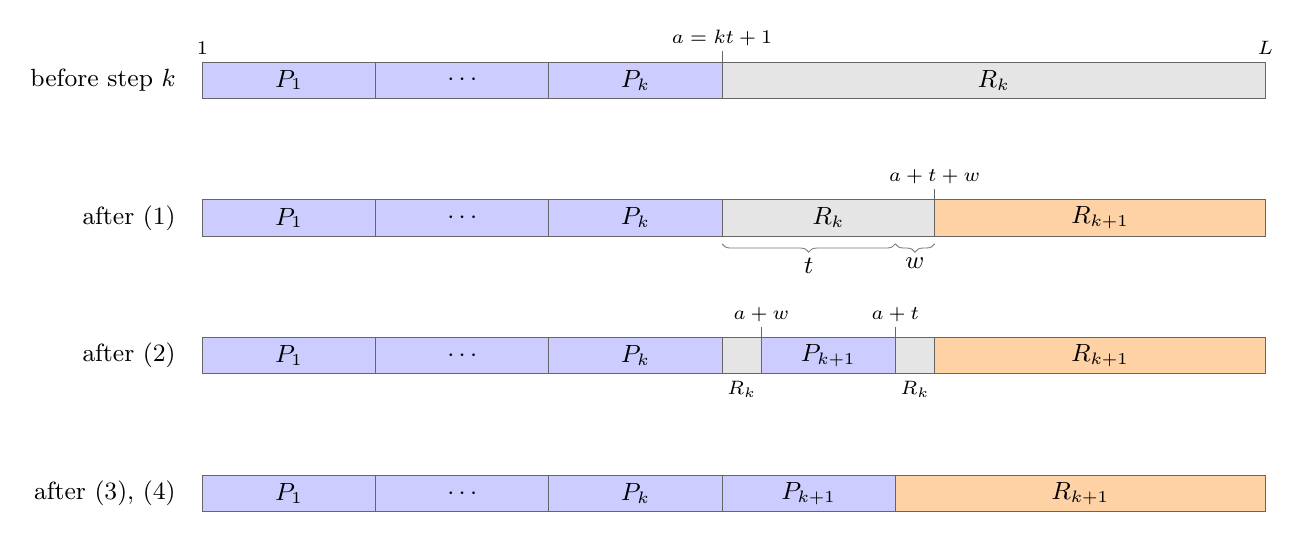
\begin{tikzpicture}[x=1cm, y=1cm, line width=0.3pt,
    lab/.style={font=\small, inner sep=1pt},
    name/.style={font=\scriptsize, text=black!55, inner sep=1pt},
    coord/.style={font=\scriptsize, inner sep=1pt},
    seg/.style={draw=black!60, line width=0.3pt},
    P/.style={seg, fill=blue!20},
    Rk/.style={seg, fill=black!10},
    Rn/.style={seg, fill=orange!35},
    brace/.style={decorate, decoration={brace, mirror, amplitude=3pt}}]
  \def\t{2.2}\def\w{0.5}\def\L{13.5}
  \def\a{6.6}      % a = k t + 1, the first site of block k+1 (3 t)
  \def\h{0.46}     % bar height
  \def\dy{1.75}    % row spacing
  \begin{scope}[yshift=0cm]
    \node[lab, anchor=east] at (-0.3, 0.5*\h) {before step \(k\)};
    \fill[P] (0, 0) rectangle (\t, \h);
    \fill[P] (\t, 0) rectangle (2*\t, \h);
    \fill[P] (2*\t, 0) rectangle (\a, \h);
    \fill[Rk] (\a, 0) rectangle (\L, \h);
    \node[lab] at (0.5*\t, 0.5*\h) {\(P_1\)};
    \node[lab] at (1.5*\t, 0.5*\h) {\(\cdots\)};
    \node[lab] at (2.5*\t, 0.5*\h) {\(P_k\)};
    \node[lab] at ({0.5*(\a+\L)}, 0.5*\h) {\(R_k\)};
    \node[coord, anchor=south] at (0, \h+0.05) {\(1\)};
    \node[coord, anchor=south] at (\L, \h+0.05) {\(L\)};
    \draw[black!60] (\a, \h) -- (\a, \h+0.14);
    \node[coord, anchor=south] at (\a, \h+0.16) {\(a=kt+1\)};
  \end{scope}
  \begin{scope}[yshift=-\dy cm]
    \node[lab, anchor=east] at (-0.3, 0.5*\h) {after (1)};
    \fill[P] (0, 0) rectangle (\t, \h);
    \fill[P] (\t, 0) rectangle (2*\t, \h);
    \fill[P] (2*\t, 0) rectangle (\a, \h);
    \fill[Rk] (\a, 0) rectangle (\a+\t+\w, \h);
    \fill[Rn] (\a+\t+\w, 0) rectangle (\L, \h);
    \node[lab] at (0.5*\t, 0.5*\h) {\(P_1\)};
    \node[lab] at (1.5*\t, 0.5*\h) {\(\cdots\)};
    \node[lab] at (2.5*\t, 0.5*\h) {\(P_k\)};
    \node[lab] at ({\a+0.5*(\t+\w)}, 0.5*\h) {\(R_k\)};
    \node[lab] at ({0.5*(\a+\t+\w+\L)}, 0.5*\h) {\(R_{k+1}\)};
    \draw[black!60] (\a+\t+\w, \h) -- (\a+\t+\w, \h+0.14);
    \node[coord, anchor=south] at (\a+\t+\w, \h+0.16) {\(a+t+w\)};
    \draw[brace, black!55] (\a, -0.1) -- (\a+\t, -0.1)
      node[lab, midway, below=4pt, text=black] {\(t\)};
    \draw[brace, black!55] (\a+\t, -0.1) -- (\a+\t+\w, -0.1)
      node[lab, midway, below=4pt, text=black] {\(w\)};
  \end{scope}
  \begin{scope}[yshift=-2*\dy cm]
    \node[lab, anchor=east] at (-0.3, 0.5*\h) {after (2)};
    \fill[P] (0, 0) rectangle (\t, \h);
    \fill[P] (\t, 0) rectangle (2*\t, \h);
    \fill[P] (2*\t, 0) rectangle (\a, \h);
    \fill[Rk] (\a, 0) rectangle (\a+\w, \h);
    \fill[P] (\a+\w, 0) rectangle (\a+\t, \h);
    \fill[Rk] (\a+\t, 0) rectangle (\a+\t+\w, \h);
    \fill[Rn] (\a+\t+\w, 0) rectangle (\L, \h);
    \node[lab] at (0.5*\t, 0.5*\h) {\(P_1\)};
    \node[lab] at (1.5*\t, 0.5*\h) {\(\cdots\)};
    \node[lab] at (2.5*\t, 0.5*\h) {\(P_k\)};
    \node[lab] at ({\a+0.5*(\t+\w)}, 0.5*\h) {\(P_{k+1}\)};
    \node[lab] at ({0.5*(\a+\t+\w+\L)}, 0.5*\h) {\(R_{k+1}\)};
    \node[coord, anchor=north] at (\a+0.5*\w, -0.06) {\(R_k\)};
    \node[coord, anchor=north] at (\a+\t+0.5*\w, -0.06) {\(R_k\)};
    \draw[black!60] (\a+\w, \h) -- (\a+\w, \h+0.14);
    \node[coord, anchor=south] at (\a+\w, \h+0.16) {\(a+w\)};
    \draw[black!60] (\a+\t, \h) -- (\a+\t, \h+0.14);
    \node[coord, anchor=south] at (\a+\t, \h+0.16) {\(a+t\)};
  \end{scope}
  \begin{scope}[yshift=-3*\dy cm]
    \node[lab, anchor=east] at (-0.3, 0.5*\h) {after (3), (4)};
    \fill[P] (0, 0) rectangle (\t, \h);
    \fill[P] (\t, 0) rectangle (2*\t, \h);
    \fill[P] (2*\t, 0) rectangle (\a, \h);
    \fill[P] (\a, 0) rectangle (\a+\t, \h);
    \fill[Rn] (\a+\t, 0) rectangle (\L, \h);
    \node[lab] at (0.5*\t, 0.5*\h) {\(P_1\)};
    \node[lab] at (1.5*\t, 0.5*\h) {\(\cdots\)};
    \node[lab] at (2.5*\t, 0.5*\h) {\(P_k\)};
    \node[lab] at (\a+0.5*\t, 0.5*\h) {\(P_{k+1}\)};
    \node[lab] at ({0.5*(\a+\t+\L)}, 0.5*\h) {\(R_{k+1}\)};
  \end{scope}
\end{tikzpicture}

\end{adjustbox}
\caption{One step of the sweep (for $k\ge1$): the word before the step, after the birth of $R_{k+1}$, after the birth of $P_{k+1}$, and after the two bands of $R_k$ have been dissolved.}\label{fig:sweep-step}
\end{figure*}

\begin{construction}[The sweep]\label{con:sweep}
Initially, a single party $R_0$ holds the entire sheet. For $k=0,1,\dots,k_*-1$, let
$a=kt+1$ be the first site of block $B_{k+1}$, and starting from the ownership word $P_1|\cdots|P_k|R_k$:
\begin{enumerate}[leftmargin=2em]
\item[(1)] Birth $R_{k+1}$ on $[a+t+w,L]$ inside $R_k$.
\item[(2)] Birth $P_{k+1}$ on $[a+w,a+t-1]$ inside $R_k$.
\item[(3)] Dissolve the band $[a,a+w-1]$ (owned by $R_k$) between $C=P_k$
and $B=P_{k+1}$ using Construction~\ref{con:band}; if $k=0$, let the band die directly
into $P_1$.
\item[(4)] Dissolve the band $[a+t,a+t+w-1]$ (owned by $R_k$) between
$C=P_{k+1}$ and $B=R_{k+1}$ using Construction~\ref{con:band}.
\end{enumerate}
After step $k_*-1$, set $P_{k_*+1}=R_{k_*}$, which owns the final block $B_{k_*+1}$.
\end{construction}

\begin{proposition}[Properties of the sweep]\label{prop:sweep}
For all sufficiently large $L$, Construction~\ref{con:sweep} defines a
distributed construction with the following properties:
\begin{enumerate}[leftmargin=2em]
\item There are $2k_*+1\le 2L$ parties. The initial state is a product state across
parties: $R_0$ holds $\Om$ on the main sheet, and every auxiliary copy of $\Om$ is initialised
privately at the party $C$ of the corresponding band dissolution.
\item There are at most $20k_*\le 2L$ non-private gates. Each involves at
most three parties and is admissible with one shared vector or covector
per monomial. Each party participates in at most $40$ non-private gates
over its lifetime.
\item The final vector $\Psi$ satisfies $\norm\Psi\le1$ and
$\norm{\Psi-\Om\otimes\Xi}\le 26\,L^{-11}$, where $\Xi$ is the tensor
product of the retired auxiliary copies of $\Om$ in their final registers
and $\norm\Xi=1$. At the end of the sweep, party $P_i$ owns precisely the raw registers
of block $B_i$, of dimension $q^{\abs{B_i}}\le q^{4t}=L^{O(1)}$, and no other
party owns any raw register.
\end{enumerate}
\end{proposition}
\begin{proof}
At the start of step $k$, the ownership word is $P_1|\cdots|P_k|R_k$, with $R_k$ owning
$[a,L]$ for $a=kt+1$. Move (1) modifies $[a+t+w,L]$ with non-$R_k$ region
$E=[1,a-1]$ at distance $t+w$; move (2) modifies $[a+w,a+t-1]$ with non-$R_k$ region
$E=[1,a-1]\cup[a+t+w,L]$ at distance $w$. Both moves are valid births by
Lemma~\ref{lem:birth} and Lemma~\ref{lem:logsep}. Afterwards, $R_k$ owns
only the two bands $[a,a+w-1]$ and $[a+t,a+t+w-1]$. In (3), $C=P_k$ owns
block $B_k$ of length $t=20w\ge8w$ to the left of $a$, and $B=P_{k+1}$ owns
$[a+w,a+t-1]$ of length $19w\ge2w$, so Lemma~\ref{lem:band} applies
(when $k=0$, the direct death of $[1,w]$ into $P_1$ has non-$P_1$ region $E=[t+1,L]$ at distance
$t-w\ge w$). In (4), $C=P_{k+1}$ owns $[a+w,a+t-1]$ of length $19w\ge8w$ and
$B=R_{k+1}$ owns $[a+t+w,L]$ of length at least $3t-w\ge2w$, so Lemma~\ref{lem:band} again applies. Step $k$ concludes with
the word $P_1|\cdots|P_{k+1}|R_{k+1}$. The distinct parties are $R_0,\dots,R_{k_*}$
and $P_1,\dots,P_{k_*}$, with $P_{k_*+1}=R_{k_*}$. Each step uses at most $2+2\cdot8=18\le20$ moves, giving at most $20k_*$ moves in total, and the final
block has length in $[3t,4t)$.

For participation counts, $R_k$ participates only in step $k-1$ (as the newborn party in (1)
and as $B$ in (4)) and in step $k$ (as $P_\circ$ in (1) and (2), and as $A$ in (3) and
(4)); similarly, $P_k$ participates only in step $k-1$ (born in (2), acting as $B$ in (3) and $C$ in (4))
and in step $k$ (acting as $C$ in (3)). Because each band dissolution consists of seven births or deaths and one
private exchange, no party participates in more than $2\cdot(2+2\cdot8)=36\le40$ gates.
Every birth or death is a single two-party gate with one shared
vector or covector, while every exchange is purely private.

For the error bound, each move maps the current state vector to within the stated
error of the updated reference vector, which is the tensor product of $\Om$
on the main sheet and $\Om$ on each active or retired auxiliary sheet in canonical
coordinates (Lemmas~\ref{lem:birth} and~\ref{lem:exchange}; retired auxiliary sheets
remain unit-norm spectators). Telescoping the product of contractions bounds
the total error by the sum of the per-move errors: two births and
two band dissolutions per step contribute at most $(2+2\cdot12)L^{-12}$, so the cumulative error over $k_*$ steps
is at most $26k_*L^{-12}\le 26L^{-11}$. Since the initial vector has unit norm and every gate is a
contraction, $\norm\Psi\le1$.
\end{proof}

\begin{figure*}[t]
\centering
\begin{adjustbox}{max width=\linewidth}
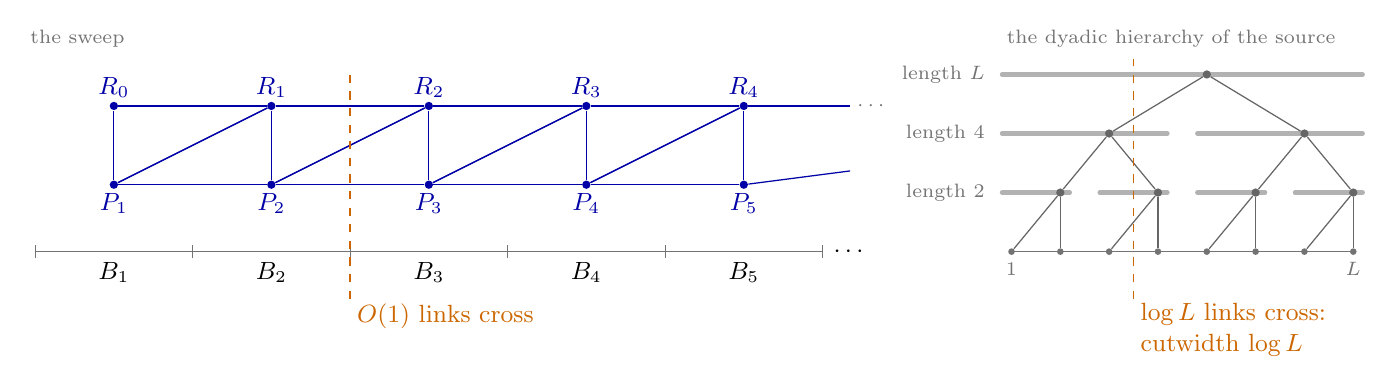
\begin{tikzpicture}[x=1cm, y=1cm, line width=0.3pt,
    lab/.style={font=\small, inner sep=1pt},
    annot/.style={font=\scriptsize, text=black!55, inner sep=1pt},
    party/.style={circle, fill=blue!65!black, inner sep=0pt, minimum size=3pt},
    link/.style={draw=blue!65!black, line width=0.45pt},
    site/.style={circle, fill=black!55, inner sep=0pt, minimum size=2.4pt},
    dnode/.style={circle, fill=black!60, inner sep=0pt, minimum size=3pt},
    dlink/.style={draw=black!60, line width=0.45pt},
    bar/.style={draw=black!30, line width=1.6pt, line cap=round},
    cut/.style={dashed, color=orange!80!black, line width=0.5pt}]
  \def\b{2.0}\def\yP{0.85}\def\yR{1.85}
  \node[annot, anchor=south west] at (-0.1, 2.55) {the sweep};
  \draw[black!55] (0, 0) -- (5*\b, 0);
  \foreach \i in {0,...,5} { \draw[black!55] (\i*\b, 0.08) -- (\i*\b, -0.08); }
  \foreach \i in {1,...,5} {
    \node[lab, anchor=north] at ({(\i-0.5)*\b}, -0.1) {\(B_{\i}\)};
  }
  \node[lab, anchor=west] at (5*\b + 0.1, 0) {\(\cdots\)};
  \foreach \i in {1,...,5} {
    \node[party] (P\i) at ({(\i-0.5)*\b}, \yP) {};
    \node[lab, anchor=north, text=blue!65!black] at ({(\i-0.5)*\b}, \yP-0.07) {\(P_{\i}\)};
  }
  \foreach \k in {0,...,4} {
    \pgfmathtruncatemacro{\j}{\k+1}
    \node[party] (R\k) at ({(\j-0.5)*\b}, \yR) {};
    \node[lab, anchor=south, text=blue!65!black] at ({(\j-0.5)*\b}, \yR+0.07) {\(R_{\k}\)};
  }
  \draw[link] (P1) -- (R0);
  \draw[link] (R0) -- (R1);
  \draw[link] (P1) -- (R1);
  \foreach \k in {1,...,4} {
    \pgfmathtruncatemacro{\j}{\k+1}
    \draw[link] (P\k) -- (R\k);
    \draw[link] (P\j) -- (R\k);
    \draw[link] (P\k) -- (P\j);
    \ifnum\k<4
      \draw[link] (R\k) -- (R\j);
      \draw[link] (P\j) -- (R\j);
    \fi
  }
  \draw[link] (R4) -- (5*\b + 0.35, \yR);
  \draw[link] (P5) -- (5*\b + 0.35, {\yP + 0.5*(\yR-\yP)*0.35/\b*2});
  \node[annot, anchor=west] at (5*\b + 0.4, \yR) {\(\cdots\)};
  \draw[cut] (2*\b, -0.6) -- (2*\b, 2.3);
  \node[lab, anchor=north west, text=orange!80!black] at (2*\b + 0.05, -0.62) {\(O(1)\) links cross};
  \begin{scope}[xshift=12.4cm]
    \def\s{0.62}\def\h{0.75}
    \node[annot, anchor=south west] at (-0.1, 2.55) {the dyadic hierarchy of the source};
    \draw[black!55] (0, 0) -- (7*\s, 0);
    \foreach \i in {1,...,8} {
      \node[site] (S\i) at ({(\i-1)*\s}, 0) {};
    }
    \node[annot, anchor=north] at (0, -0.1) {\(1\)};
    \node[annot, anchor=north] at (7*\s, -0.1) {\(L\)};
    \foreach \a/\c/\p in {1/2/2, 3/4/4, 5/6/6, 7/8/8} {
      \draw[bar] ({(\a-1)*\s - 0.12}, \h) -- ({(\c-1)*\s + 0.12}, \h);
      \node[dnode] (D\a\c) at ({(\p-1)*\s}, \h) {};
      \draw[dlink] (D\a\c) -- (S\a);
      \draw[dlink] (D\a\c) -- (S\c);
    }
    \foreach \a/\m/\n/\c/\p in {1/2/3/4/3, 5/6/7/8/7} {
      \draw[bar] ({(\a-1)*\s - 0.12}, 2*\h) -- ({(\c-1)*\s + 0.12}, 2*\h);
      \node[dnode] (D\a\c) at ({(\p-1)*\s}, 2*\h) {};
      \draw[dlink] (D\a\c) -- (D\a\m);
      \draw[dlink] (D\a\c) -- (D\n\c);
    }
    \draw[bar] (-0.12, 3*\h) -- (7*\s + 0.12, 3*\h);
    \node[dnode] (D18) at (4*\s, 3*\h) {};
    \draw[dlink] (D18) -- (D14);
    \draw[dlink] (D18) -- (D58);
    \node[annot, anchor=east] at (-0.3, \h) {length \(2\)};
    \node[annot, anchor=east] at (-0.3, 2*\h) {length \(4\)};
    \node[annot, anchor=east] at (-0.3, 3*\h) {length \(L\)};
    \draw[cut] (2.5*\s, -0.6) -- (2.5*\s, 2.45);
    \node[lab, anchor=north west, text=orange!80!black, align=left] at (2.5*\s + 0.05, -0.62)
      {\(\log L\) links cross:\\ cutwidth \(\log L\)};
  \end{scope}
\end{tikzpicture}

\end{adjustbox}
\caption{Left: the party graph of the sweep placed on the chain; a bounded number of links cross any bond. Right: a dyadic hierarchy drawn on a line, where every scale contributes a link across the middle bond.}\label{fig:party-graph}
\end{figure*}

\begin{remark}[Why small-patch rewrites are unneeded]
In two dimensions \cite[Section~4]{PP}, squares of side length below $K_0\log L$
must be repainted by ``small-patch rewrites'' using finite-rank cylinder
projections of polynomial rank. In one dimension, the final owners $P_i$ hold
blocks of $O(\log L)$ consecutive sites whose Hilbert-space dimension
$q^{\abs{B_i}}=q^{O(\log L)}$ is already polynomial in $L$, and the compression
theorem of Section~\ref{sec:compression} accepts polynomial-dimensional physical
outputs directly. Factoring each block tensor into single-site matrix-product
tensors is then a routine singular value decomposition (Section~\ref{sec:routing}).
This is the second reason why the adaptive patch constraints of \cite{PP} are
unneeded on a chain.
\end{remark}

\section{Compression and column extraction}\label{sec:compression}

\begin{inwords}
The sweep protocol is a sequence of linear contractions followed by a partial
trace over all registers except the physical block outputs. Its non-private
gates still rely on shared bipartite vectors of enormous dimension (such as
purifications of half-chain marginals). To compress these virtual links to
polynomial dimension, the density-compression theorem replaces each shared
source operator $\ket\eta\bra{\tilde\eta}$ in the density calculation
$\rho=\Tr_{\mathrm{private}}\ket\Psi\bra\Psi$ with the sample average of $k$
independent random product operators $U_j\otimes V_j$ built from its Schmidt
decomposition and standard complex Gaussian coefficients. For a polynomial
sample size $k$, the physical output density changes by at most $L^{-p}$ in
trace norm. Expanding the error according to the subset of slots where a
centred correction $\widehat X-X$ acts, each corrected slot involves only its
two endpoint parties, and bounded participation ensures that only a bounded
number of gates per corrected slot must be expanded into monomials; a
Gaussian second-moment computation with Schatten--Hölder then shows that a
term with $s$ corrections has expected trace norm at most $k^{-s/2}$ times a
fixed polynomial per correction. Because this estimate depends only on the
trace-one Schmidt probability weights and the combinatorial participation
bounds, it is completely independent of the private Hilbert-space dimensions
and of the Schmidt ranks of the shared states. Fixing a deterministic
realisation produces an operator tensor network $\sigma$ with one node per
party and polynomial-dimensional links between parties that shared a gate.
Extracting a single product-basis column $\sigma\ket z$ then converts
$\sigma$ into a ket tensor network with the same virtual links, which
approximates the ground vector after normalisation. The theorem and its
proof are not geometric and carry over without change; we restate the
theorem in the form used here and sketch the estimate.
\end{inwords}

\precisely
\begin{theorem}[Density compression, {\cite[Theorem~5.2]{PP}}]\label{thm:compression}
Consider a family of distributed constructions indexed by $L\ge2$ such
that: the numbers of parties and gates are uniformly polynomial; the
initial vector is a product of normalised private vectors; every gate is
a contraction; each non-private gate involves at most $b$ parties and each
party participates in at most $b$ non-private gates; each non-private gate
is admissible with uniformly polynomial bounds; and the intended physical
output of each party has uniformly polynomial dimension, everything else
being traced out. Let $\rho$ be the physical output density (positive,
trace at most one). For every fixed $p>0$ there is an operator tensor
network $\sigma$ with one node per party, a bounded number of links at
each node, each link joining two parties that participate in a common
non-private gate, uniformly polynomial link dimensions, and
\[
 \norm{\sigma-\rho}_1\le L^{-p}.
\]
The constants depend only on $p$, $b$, and the uniform polynomial bounds,
not on private dimensions or on the Schmidt ranks of shared vectors.
\end{theorem}
\begin{proof}[Sketch]
First eliminate shared covectors: a covector $\bra\eta$ on a pair of
registers is replaced by appending $m-1$ copies of $\eta$ and averaging over the
$m$ cyclic permutations of the $m$ pair registers, forming a contraction $T_m$ with
$\norm{T_m-\ket\eta^{\otimes m}\bra\eta}=m^{-1/2}$. Attaching a common fixed
garbage vector in every branch approximates a gate with $K$ monomials, each containing at
most $r$ covectors, to within operator-norm error
$rm^{-1/2}\sum\abs{c_\xi}$ by a gate with $Km^r$ monomials using shared
vectors only. Choosing $m$ polynomially large makes this error at most
$\epsilon/(8M)$ per gate, where $M$ is the number of non-private gates.

Next, in the density calculation, each source operator $X=\ket\eta\bra{\tilde\eta}$
with Schmidt decompositions $(\lambda_a,u_a,v_a)$ and $(\mu_c,\tilde u_c,\tilde v_c)$
is replaced by $\widehat X=\frac1k\sum_{j=1}^kU_j\otimes V_j$, where
$U_j=\sum_{a,c}(\lambda_a\mu_c)^{1/4}g^{(j)}_{ac}\ket{u_a}\bra{\tilde u_c}$ and
$V_j=\sum_{b,d}(\lambda_b\mu_d)^{1/4}\overline{g^{(j)}_{bd}}\ket{v_b}\bra{\tilde v_d}$
for independent standard complex Gaussians $g^{(j)}_{ac}$. Then
$\E\widehat X=X$, and by the Gaussian pairing formula the centred coefficients of $\Delta=\widehat X-X$ have
diagonal covariance $k^{-1}\sqrt{\lambda_a\lambda_b\mu_c\mu_d}$. Expanding the product over all $N$ source
slots gives $\widehat\rho-\rho'=\sum_{\varnothing\ne S}F_S$, where $S$ indexes
the slots carrying a correction $\Delta$. For $\abs S=s$, the corrected slots touch
at most $2s$ endpoint parties, which participate in at most $2bs$ gates; expand only
those gates into monomials and fix the physical basis entries at those
parties, at a total weighted cost of at most $Q(L)^s$ for a fixed polynomial $Q$.
For each fixed choice, the network factors into an affected side
(holding the corrected endpoints as free inputs) and an exterior side, connected
only by the exact shared vectors crossing between them, with Schmidt
probability matrices $\tau$ and $\tilde\tau$. The affected contractions form a
block operator $O$ of norm at most one, the corrected coefficients $z_{il}$
have covariance $k^{-s}\sqrt{p_i\tilde p_l}\,\delta\delta$, and the operator fed into the exterior
is $Z=\sum_{il}z_{il}\tau^{1/2}O_{li}^{\mathsf T}\tilde\tau^{1/2}$.
Applying the Schatten--Hölder inequality with exponents $(4,2,4)$ and the trace-one weights $\tau,\tilde\tau$ gives
$\norm Z_1\le\norm{\sum_{il}z_{il}\tilde\tau^{1/4}O_{li}\tau^{1/4}}_2$, whose expected
square is $k^{-s}\norm{\widetilde R^{1/4}OR^{1/4}}_2^2\le k^{-s}$ with
$R=\mathrm{diag}(p_i)\otimes\tau$ and $\widetilde R=\mathrm{diag}(\tilde p_l)\otimes\tilde\tau$.
Because the exterior contractions and the physical matrix units are trace-norm contractions,
$\E\norm{F_S}_1\le Q(L)^sk^{-s/2}$ and hence
$\E\norm{\widehat\rho-\rho'}_1\le(1+Q(L)k^{-1/2})^N-1\le\epsilon/4$ for a
polynomial sample size $k$. Fixing a realisation of the Gaussian variables yields $\sigma$: the monomial
index of each gate is shared along a star linking its participating parties, and each
slot's sample index $j\in\{1,\dots,k\}$ is shared between its two endpoint parties, while all private
contractions, private state preparations, and final private traces are
absorbed into each party's local node tensor.
\end{proof}

\begin{figure}[t]
\centering
\begin{adjustbox}{max width=\linewidth}
\(\begin{tenkz}[size=l, rows={wire,wire}, cols=2, bonds=none]
  \tn[at=(1,1), skin=box, wide=2, ports={90@1:physical, 90@2:physical}]{\eta}
  \tn[at=(2,1), skin=box, wide=2, ports={270@1:physical, 270@2:physical}]{\tilde\eta^{\,\dagger}}
\end{tenkz}
=\mathbb E\,\frac1k
\begin{tenkz}[size=l, rows={wire}, cols=2, bonds=none]
  \tn[at=(1,1), name=u, skin=box, ports={0:virtual, 90:physical, 270:physical}]{U_j}
  \tn[at=(1,2), name=w, skin=box, ports={180:virtual, 90:physical, 270:physical}]{V_j}
  \tnbond[name=j]{u.0}{w.180}
\end{tenkz}\)

\end{adjustbox}
\caption{The random replacement of one pair source: the operator $\ket\eta\bra{\tilde\eta}$ equals the expectation of $\frac1k\sum_j U_j\otimes V_j$, the two factors joined by the sample index $j$.}\label{fig:source-sampling}
\end{figure}

\begin{lemma}[Column extraction, {\cite[Lemma~8.1]{PP}}]\label{lem:column}
Let $\Om$ be a unit vector on a finite tensor product and $\sigma$ an
operator with $\norm{\sigma-\ket\Om\bra\Om}_1\le\eta<1$. Then some
product-basis column $v=\sigma\ket z$ is nonzero and satisfies
$\min_\theta\norm{v/\norm v-\e^{i\theta}\Om}\le2\eta$. Fixing a column in an
operator tensor network leaves all virtual dimensions unchanged.
\end{lemma}
\begin{proof}
Let $E=\sigma-\ket\Om\bra\Om$ and $a_z=\langle\Om|z\rangle$. Since
$\sum_z\norm{E\ket z}^2=\norm E_2^2\le\eta^2$ and $\sum_z\abs{a_z}^2=1$,
there exists a product-basis label $z$ with $a_z\ne0$ and $\norm{E\ket z}\le\eta\abs{a_z}$. For this $z$,
the rescaled column $w=v/a_z$ satisfies $\norm{w-\Om}\le\eta$, so $w\ne0$ and
$\norm{w/\norm w-\Om}\le2\eta$. Fixing the bra index at every node contracts
only physical legs, leaving all virtual bond dimensions unchanged.
\end{proof}

\begin{figure}[t]
\centering
\begin{adjustbox}{max width=\linewidth}
\(\begin{tenkz}[size=l, rows={wire,wire}, cols=3, bonds=none]
  \tn[at=(1,1), name=a, skin=box, ports={0:virtual, 90:physical, 270:physical}]{\sigma}
  \tn[at=(1,2), name=b, skin=box, ports={180:virtual, 0:virtual, 90:physical, 270:physical}]{\sigma}
  \tn[at=(1,3), name=c, skin=box, ports={180:virtual, 90:physical, 270:physical}]{\sigma}
  \tn[at=(2,1), name=za, skin=tri, ports={90:physical}]{}
  \tn[at=(2,2), name=zb, skin=tri, ports={90:physical}]{}
  \tn[at=(2,3), name=zc, skin=tri, ports={90:physical}]{}
  \tnbond{a.0}{b.180} \tnbond{b.0}{c.180}
  \tnwire{a.270}{za.90} \tnwire{b.270}{zb.90} \tnwire{c.270}{zc.90}
\end{tenkz}
=
\begin{tenkz}[size=l, rows={wire}, cols=3, bonds=none]
  \tn[at=(1,1), name=a, skin=box, ports={0:virtual, 90:physical}]{v}
  \tn[at=(1,2), name=b, skin=box, ports={180:virtual, 0:virtual, 90:physical}]{v}
  \tn[at=(1,3), name=c, skin=box, ports={180:virtual, 90:physical}]{v}
  \tnbond{a.0}{b.180} \tnbond{b.0}{c.180}
\end{tenkz}\)

\end{adjustbox}
\caption{Column extraction: fixing the input legs of the operator chain by a product-basis covector gives a ket chain with the same bonds.}\label{fig:column}
\end{figure}

\section{Assembly on the chain}\label{sec:routing}

\begin{inwords}
We now apply density compression and column extraction to the sweep protocol
and route the resulting party network along the chain. The parties of the
sweep are the block owners $P_i$, whose physical outputs are the
$q^{\abs{B_i}}$-dimensional block registers, and the remainder parties $R_k$,
which have no physical outputs. Every link in the compressed party network
connects two parties that shared a non-private gate, and by construction
those parties belong to the same or adjacent sweep steps. Placing the node of
$R_k$ alongside block $B_{k+1}$ ensures that the chain cut between blocks
$B_i$ and $B_{i+1}$ is crossed only by links among the boundedly many parties
attached to the four nearest blocks. This bounded congestion implies that each
inter-block bond has dimension equal to a bounded product of polynomial link
dimensions. Column extraction first converts the compressed operator network
into a ket network on the blocks; sequential singular value decompositions
across the sites within each block then split each block tensor into
single-site tensors whose internal bond dimensions are at most
$q^{\abs{B_i}}$ times the inter-block bond dimension, which remains
polynomial in $L$. Chains shorter than the threshold $L_0$ are represented
exactly.
\end{inwords}

\precisely
\begin{proof}[Proof of Theorem~\ref{thm:B}]
Choose $L_0$ large enough for Proposition~\ref{prop:sweep} and for the
inequalities below to hold; for $2\le L<L_0$, every state vector on $\Lam$ admits an exact
matrix product state representation of bond dimension at most $q^{\lfloor L/2\rfloor}\le
q^{L_0/2}$, which is absorbed into the prefactor $C$. Assume henceforth that $L\ge L_0$.

By Proposition~\ref{prop:sweep}(3) and the inequality
$\norm{\ket u\bra u-\ket v\bra v}_1\le2\norm{u-v}$ for vectors of norm at
most one, the physical output density
$\rho=\Tr_{\mathrm{private}}\ket\Psi\bra\Psi$ satisfies
$\norm{\rho-\ket\Om\bra\Om}_1\le 52L^{-11}$. The sweep satisfies the
hypotheses of Theorem~\ref{thm:compression} with participation bound $b=40$ and physical
output dimensions at most $q^{4t}\le L^{80D_{24}\log q+1}$. Applying Theorem~\ref{thm:compression} with target
accuracy $L^{-5}$ yields an operator tensor network $\sigma$ on the party
graph with $\norm{\sigma-\ket\Om\bra\Om}_1\le L^{-5}+52L^{-11}\le2L^{-5}$,
bounded node degree, and link dimensions at most $C_1L^{r}$. By
Lemma~\ref{lem:column}, some product-basis column of $\sigma$ is a nonzero ket tensor network $v$ with the
same virtual links satisfying $\min_\theta\norm{v/\norm v-\e^{i\theta}\Om}\le4L^{-5}\le L^{-1}$.

\emph{Placement and routing.} Assign $P_i$ to block $B_i$ and $R_k$ to block $B_{k+1}$, and
contract the two party nodes assigned to each block into a single block node (links between them
cross no inter-block cut). By the proof of
Proposition~\ref{prop:sweep}, any two parties sharing a gate belong to
$\{P_k,P_{k+1},R_k,R_{k+1}\}$ for some step $k$, and are therefore assigned to the same
or adjacent blocks (our bound below accommodates blocks up to two apart). The cut between blocks $B_i$ and $B_{i+1}$ is thus
crossed only by links incident to parties assigned to blocks
$B_{i-1},\dots,B_{i+2}$. There are at most $8$ such parties, each of degree at most
$5\cdot40$ (at most two star links and three sample links per three-party
gate), so at most $\chi:=1600$ links cross any inter-block cut. Route each link along the chain
between its endpoint blocks and bundle the links crossing each inter-block cut into a single
bond index of dimension at most $(C_1L^r)^{\chi}$. The tensor at block $B_i$ is
then a linear map from its left and right inter-block bond spaces to the block's
physical Hilbert space $\cH_{B_i}$ of dimension at most $q^{4t}$. Writing
$B_i=\{x_1<\dots<x_n\}$, perform successive singular value decompositions
across the internal cuts $x_1|x_2\cdots x_n$, $x_1x_2|x_3\cdots x_n$, \dots,
treating the left and right inter-block bond indices as external legs attached to
$x_1$ and $x_n$. The resulting single-site tensors have internal
bond dimensions at most $\min\{q^{j}(C_1L^r)^\chi,\ q^{n-j}(C_1L^r)^\chi\}\le
q^{2t}(C_1L^r)^{\chi}$, while the inter-block bonds remain unchanged. Thus $v$ is a
matrix product state on $\Lam$ with open boundary conditions and bond
dimension at most $q^{2t}(C_1L^r)^\chi\le CL^{c}$, with exponent
$c=40D_{24}\log q+r\chi$.
\end{proof}

\begin{figure*}[t]
\centering
\begin{adjustbox}{max width=\linewidth}
\(\displaystyle \begin{tenkz}[size=l, rows={wire,wire}, cols=4, bonds=none]
    \tn[at=(2,1), skin=box, wide=4, name=b,
        ports={180:virtual:$(C_1L^r)^{\chi}$, 0:virtual:$(C_1L^r)^{\chi}$,
               90@1:physical, 90@2:physical, 90@3:physical, 90@4:physical}]{B_i}
    \tn[at=(1,1), skin=none, name=p1, ports={270:physical, 90:physical:$x_1$}]{}
    \tn[at=(1,2), skin=none, name=p2, ports={270:physical, 90:physical:$x_2$}]{}
    \tn[at=(1,3), skin=none, name=p3, ports={270:physical, 90:physical:$x_3$}]{}
    \tn[at=(1,4), skin=none, name=p4, ports={270:physical, 90:physical:$x_4$}]{}
    \tnwire{b.90@1}{p1.270} \tnwire{b.90@2}{p2.270}
    \tnwire{b.90@3}{p3.270} \tnwire{b.90@4}{p4.270}
  \end{tenkz}
  \;=\;
  \begin{tenkz}[size=l, rows={wire,wire}, cols=7, bonds=none]
    \tn[at=(2,1), name=a1, skin=box, ports={180:virtual:$(C_1L^r)^{\chi}$, 0:virtual, 90:physical}]{A^{[x_1]}}
    \tn[at=(2,3), name=a2, skin=box, ports={180:virtual, 0:virtual, 90:physical}]{A^{[x_2]}}
    \tn[at=(2,5), name=a3, skin=box, ports={180:virtual, 0:virtual, 90:physical}]{A^{[x_3]}}
    \tn[at=(2,7), name=a4, skin=box, ports={180:virtual, 0:virtual:$(C_1L^r)^{\chi}$, 90:physical}]{A^{[x_4]}}
    \tn[at=(1,1), skin=none, name=q1, ports={270:physical, 90:physical:$x_1$}]{}
    \tn[at=(1,3), skin=none, name=q2, ports={270:physical, 90:physical:$x_2$}]{}
    \tn[at=(1,5), skin=none, name=q3, ports={270:physical, 90:physical:$x_3$}]{}
    \tn[at=(1,7), skin=none, name=q4, ports={270:physical, 90:physical:$x_4$}]{}
    \tnwire{a1.90}{q1.270} \tnwire{a2.90}{q2.270} \tnwire{a3.90}{q3.270} \tnwire{a4.90}{q4.270}
    \tnbond[name=d1]{a1.0}{a2.180} \tnbond[name=d2]{a2.0}{a3.180} \tnbond[name=d3]{a3.0}{a4.180}
    \tnmark[form=label, label pos=90]{on d1 0.5}{$q^{2t}(C_1L^r)^{\chi}$}
    \tnmark[form=label, label pos=90]{on d2 0.5}{$q^{2t}(C_1L^r)^{\chi}$}
    \tnmark[form=label, label pos=90]{on d3 0.5}{$q^{2t}(C_1L^r)^{\chi}$}
  \end{tenkz}\)

\end{adjustbox}
\caption{A block tensor with its two block bonds and $t$ physical legs is split into $t$ site tensors by successive singular value decompositions; the new bonds are at most $q^{2t}$ times the block-bond dimension.}\label{fig:block-to-sites}
\end{figure*}

\begin{remark}[Order of constants]
Fix $q,R,J,\Delta$. Theorem~\ref{thm:A} determines the interval entropy bound $C_{\mathrm{int}}$;
Lemma~\ref{lem:reset} at exponent $p=24$ determines $C_{24}$, which fixes $D_{24}$ and the
block length $t=20w$; the party and gate counts together with the participation bound
$b=40$ are then fixed; Theorem~\ref{thm:compression} at accuracy $L^{-5}$
fixes the covector permutation count $m$, the Gaussian sample size $k$, and
the link-dimension exponent $r$; and the congestion bound $\chi=1600$ is an absolute numerical constant.
None of these constants depends on the specific Hamiltonian $H$ or on the chain length $L$. Over the full sweep, the protocol prepares
$O(L/\log L)$ auxiliary copies of $\Om$, all held privately.
\end{remark}

\section{Discussion}\label{sec:discussion}

\begin{inwords}
\emph{Comparison with earlier one-dimensional proofs.} Hastings' proof of the
one-dimensional area law \cite{Hastings2007} shows that the half-chain
marginal has an entanglement spectrum whose tail decays exponentially beyond
rank $\exp(O(1))$ by combining a Lieb--Robinson bound, a spectral filter
that approximately projects onto the ground state, and a bound on the
approximate factorisation of the filtered state. Arad, Kitaev, Landau, and Vazirani
\cite{AKLV} replace the time-evolution filter with an approximate
ground-state projector constructed from Chebyshev polynomials of controlled
Schmidt rank, which is then amplified by bootstrapping. By contrast, the
proof of Theorem~\ref{thm:A} in Part~\ref{part:arealaw} uses no real-time
dynamics at all: the spectral gap enters only to bound the overlap of a
variationally tilted or filtered vector with the ground vector, and the entanglement
entropy is extracted directly from operator norms via Hölder's inequality, a
three-lines interpolation, and the Araki--Lieb triangle
inequality, yielding a linear $O(J/\Delta)$ scaling in the inverse gap. For
Theorem~\ref{thm:B}, this note presents two distinct constructions of the
matrix product state: the direct two-line route of Section~\ref{sec:shortcut},
which combines the marginal tail bound (Lemma~\ref{lem:tail}) with the area
law (Theorem~\ref{thm:A}) and is likewise completely free of dynamics, and
the distributed protocol route of Part~\ref{part:mps}, which invokes a
Lieb--Robinson bound in a single place (the information reset,
Lemma~\ref{lem:reset}) but in a way that has no analogue in Hastings'
construction (a two-replica swap undone by a local unitary), and otherwise
relies solely on Uhlmann-type ownership moves, random Gaussian compression,
and product-basis column extraction.

\emph{Simplifications specific to one dimension.} Three geometric features of
the line simplify the two-dimensional arguments of \cite{AL,PP}, each used in
exactly one place. First, the shell around any interval is crossed by $O(1)$
interaction terms, so the buffered discount (Lemma~\ref{lem:buffer}) costs
a constant and needs only a constant-width buffer. Second, no three interval owners ever meet at a single point on
a line, eliminating trijunctions and the associated boundary encodings in the
ownership moves (Section~\ref{sec:moves}). Third, the chain can be swept
sequentially from left to right, giving a party graph of $O(1)$ cutwidth
rather than the $\log L$ cutwidth of a dyadic tree (Section~\ref{sec:sweep}).
Everything else in \cite{AL,PP} is either unchanged or disappears.

\emph{Why the two-dimensional obstructions are genuine.} None of these three
one-dimensional shortcuts extends back to two dimensions. In two dimensions,
the Araki--Lieb closure fails because the buffer surrounding a region is a
thin annulus whose own entanglement entropy is a priori unknown; a linear
sweep fails because repainting a two-dimensional region exposes a
one-dimensional boundary along which a third owner is adjacent, necessitating
the edge-band dissolutions and trijunction treatments of \cite{PP}; and sequential
Schmidt truncation across nested cuts does not produce a two-dimensional
tensor network on the lattice. The multiscale machinery of
\cite{AL,PP} is therefore dictated by genuine two-dimensional geometric and
topological obstructions that simply do not arise on a chain.
\end{inwords}
